\section{a}

\subsection{Review and Introducing the Model}
Last time we gave a teaser about the spherical model; note that historically, the exact solution to the 2D Ising model was actually discovered first (though the spherical model is much easier to solve, which is why we discuss it first)! We work out the phase diagram of what is basically a ferromagnet.

\begin{figure}[htbp]
    \centering
    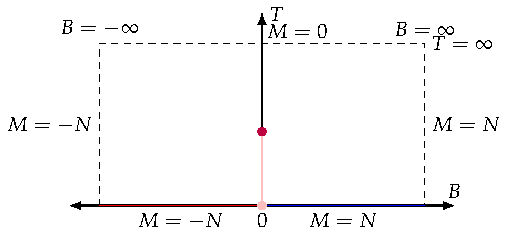
\includegraphics{Images/fig-IsingphasediagramB0.pdf}
    \caption{Phase diagram of infinite range Ising model and Spherical model.}
    \label{fig-sphericalmodelphasediagram}
\end{figure}

In 1D, we found spontaneous symmetry breaking at $B = 0, T = 0$. In the infinite range model, we found that this behaviour persists at finite temperature (with a first-order phase transition line) and culminating in a second-order phase transition point at $B = 0, T = T_c$. We studied the behaviour of the phase diagram in the vicinity of $T_c$. We observed the phenomena of universality, which in a practical sense told us that all that matters to determine the critical phenomena were the first few terms of the Taylor expansion of the free energy, and any model that produced the same coefficients have the same critical exponents - those of mean field theory. Presumably, if we found something else that was not mean field theory, it would still not depend on very much. Gordon isn't aware of a rigorous way of showing that a certain system is in a particular universality class, but even with this missing, it is thrown around in research seminars as if we understand this fully; so it is good to understand the terminology.

The spherical model is another model, and it will have the same phase diagram as the infinite range Ising model; the new thing will be that some of the critical exponents are \emph{not} mean field, which will tell us that mean field theory is not everything! Landau conjectured that mean field theory was everything, but by example we can show him to be wrong.

In the Ising model, the spins were discrete $\sigma_x = \pm 1$. In the spherical model, we lift this restriction and allow $\sigma_x \in \RR$. However there is a problem; looking at the exchange term in the Hamiltonian:
\begin{equation}
    H = -J\sum_{x, i}\sigma_x \sigma_{x + i}
\end{equation}
we see that there is no lower bound on the energy (by taking $\sigma_x \to \infty$). In order to ensure that this pathological behaviour does not occur, we introduce the constraint:
\begin{equation}
    \sigma_x \sigma_x^2 = N
\end{equation}
which tells us that on average, $\sigma_x \sim 1$. This bounds the energy from below. We also have the magnetic term, so the full Hamiltonian is:
\begin{equation}
    H = -J\sum_{x, i}\sigma_{x}\sigma_{x + i} - B \sum_x \sigma_x
\end{equation}
note that to generate correlation functions, it is sometimes useful to make $B$ site-dependent:
\begin{equation}
    H = -J\sum_{x, i}\sigma_{x}\sigma_{x + i} - \sum_x B_x\sigma_x
\end{equation}
this makes the model unsolvable, but can be useful for some analysis (e.g. allows us to take derivatives, and then we can set $B$ to a constant).

\subsection{Ground State of the Spherical Model}
Is the ground state (formally this is not a quantum mechanical system so we should say lowest-energy state, but it's hard to resist calling it this) of this model ordered? Let us include the constraint into the Hamiltonian:
\begin{equation}
    \tilde{H} = -J\sum_{x, i}\sigma_x \sigma_{x + i} - B \sum_x \sigma_x + \lambda \left(\sum_x \sigma_x^2 - N\right)
\end{equation}
The equations for the extrema are:
\begin{equation}
    -J\sum_i \left(\sigma_{x + i} + \sigma_{x - i}\right) - B + 2\lambda \sigma_x = 0
\end{equation}
\begin{equation}
    \sum_x \sigma_x^2 = N
\end{equation}
It can be argued that the ground state should be independent of $x$. To this end, let us rewrite the Hamiltonian as follows:
\begin{equation}
    H = \frac{J}{2}\sum_{x, i}\left(\sigma_{x + i} - \sigma_x\right)^2 - JD\sum_x \sigma_x^2 - B\sum_x \sigma_x + \lambda\left(\sum_x \sigma_x^2 - N\right)
\end{equation}
Now, we want to minimize the above. We have a positive function plus something else; so we want to at least get the positive term $\sum_{x, i}(\sigma_{x + i} - \sigma_x)^2$ to zero. This will not interfere with minimizing the rest because the rest of the terms only depend on a single site (so we just minimize per site). Then, we observe that to minimize $\sum_{x, i}(\sigma_{x + i} - \sigma_x)^2$, the $\sigma_x$s should be site independent. This concludes the argument. Having shown this property, we conclude that $\sigma_x^2 = 1$ (i.e. just the average value) and so we find:
\begin{equation}
    \sigma_x = \text{sign}(B), \quad \lambda = DJ + \frac{\abs{B}}{2}, U[T = 0] = -N\left(2DJ + \abs{B}\right)
\end{equation}
We see that the derivative of the energy is discontinuous at $B = 0$. We also see that the magnetization is completely determined by the sign of $B$ (so we have for $T = 0$ that $m = -1$ for $B < 0$ and $m = 1$ for $B > 0$, as we claimed). 

\subsection{Finite Temperature Spherical Model}
If we turn on $T$, we want to find the partition function:
\begin{equation}
    Z[T, B, N] = \int_{-\infty}^\infty \prod_x d\sigma_x e^{-\frac{J}{k_B T}\sum_{x, i} \sigma_x \sigma_{x  + i} + \frac{B}{k_B T}\sum_x \sigma_x}\delta(\sum_x \sigma_x^2 - N)
\end{equation}
where we have enforced the constraint by introducing a dirac delta function into the measure\footnote{Actually, note quite - we are missing the Jacobian term; but it suffices in our case to know that the Jacobian does not grow as the exponential of something, which it does not in this case, so we can neglect it}. To evaluate this, we could write the Dirac delta function as a Fourier integral:
\begin{equation}
    \delta(\sum_x \sigma_x^2 - N) = \int \frac{d\lambda}{2\pi}e^{i\lambda\left(\sum_x \sigma_x^2 - N\right)}
\end{equation}
then evaluate things via the saddle point technique. Instead of doing this - let us solve a simplified version of the model.

\subsection{Mean Spherical Model}
In this simplified version of the model, we replace the constraint $\sum_x \sigma_x^2 = N$ with the constraint that:
\begin{equation}
    \avg{\sum_x \sigma_x^2} = N
\end{equation}
i.e. the configurational average of the sum of the square of the spins is $N$. This still fixes the problem of the Hamiltonian not having a lower bound on the energy, but turns out to be easier to solve. How do we implement this constraint? What we will do is the following; add a term to the exponent:
\begin{equation}
    Z[T, B, N] = \int_{-\infty}^\infty \prod_x d\sigma_x e^{\frac{J}{k_B T}\sum_x \sigma_x \sigma_{x + i} + \frac{B}{k_B T}\sum_X \sigma_x - \mu \sum_x \sigma_x^2}
\end{equation}
In the spherical model proper this would just be adding the constant $-\mu N$ to the model and would do nothing. Here it will have a nontrivial effect. The constraint is implemented by:
\begin{equation}
    \left.-\dpd{}{\mu}\ln Z\right|_{N, T, B} = N
\end{equation}
So, let us calculate the partition function and enforce the above constraint to solve the mean spherical model.

\subsection{Interlude - Gaussian Integral}
Ok, now to solve this model, we will introduce the Gaussian integral\footnote{So long as we can diagonalize $2 \times 2$ matrices and evaluate Gaussian integrals, you're ready to be a theorist, apparently\ldots}. In the course notes the Gaussian integral result is stated but not shown. Here, let's actually walk through it. Let's rewrite the integral for the partition function as:
\begin{equation}\label{eq-Gaussianintegralstart}
    Z[T, B, N]  = \int_{-\infty}^\infty \prod_x d\sigma_x e^{-\frac{1}{2}\sum_{x, y}\sigma_x \Delta(x, y)\sigma_y + \frac{B}{k_B T}\sum_x \sigma_x}
\end{equation}
where:
\begin{equation}\label{eq-Deltaxyspherical}
    \Delta(x, y) = \frac{J}{k_B T}\sum_i\left[2\delta_{xy} - \delta_{x, y+i} - \delta_{x, y - i}\right] + 2\left(\mu - \frac{JD}{k_B T}\right)\delta_{xy}
\end{equation}
where we have written things in a bit of a special way; note that the first and last terms cancel, and the second/third terms are symmetrizing the exchange term of the Hamiltonian. Before discussing the details, let us discuss how to do the integral in Eq. \eqref{eq-Gaussianintegralstart}. We can think of $\sigma_x$ as an $N$-dimensional row vector, $\Delta(x, y)$ as an $N \times N$ matrix, and $\sigma_y$ as a column vector (and hence what appears in the exponential is a kind of matrix multiplication followed by taking an inner product). There is an exponential damping here, and one might suspect that when this dampening is supressed we have critical behaviour (and this is indeed the case). We will assume $\Delta(x, y)$ is a real and symmetric matrix (we see that this is indeed the case for Eq. \eqref{eq-Deltaxy}). We then use a theorem from linear algebra that tells us that we can diagonalize such a matrix via an orthogonal transformationL:
\begin{equation}
    \Delta(x, y) = O_{x w}\Delta_{w}\delta_{wz}O_{zy}^T
\end{equation}
where orthogonality means:
\begin{equation}
    OO^T = \II
\end{equation}
i.e. the rows are orthogonal to each other and normalized. We also have the completeness sums:
\begin{equation}
    O^T O = \II
\end{equation}
The matrix $\Delta_w \delta_{wz}$ is diagonal:
\begin{equation}
    \Delta_w \delta_{wz} = \m{\Delta_1 & 0 & \ldots & 0
    \\ 0 & \Delta_2 & \ldots & 
    \\ \vdots & & \ddots & 
    \\ 0 & & & \Delta_N}
\end{equation}
Let us therefore change integration variables:
\begin{equation}
    \sigma_x \to O_{xy}\sigma_y
\end{equation}
which has the effect on the integral:
\begin{equation}
    \int \pi_x d\sigma_x \to \int \pi_x d\sigma_x \abs{\det O}
\end{equation}
Note that:
\begin{equation}
    \det OO^T = 1 \implies (\det O)^2 = 1 \implies \det O = \pm 1 \implies \abs{\det O} = 1
\end{equation}
and so:
\begin{equation}
    \begin{split}
        \int \prod_x d\sigma_x e^{-\frac{1}{2}\sum_{xy} \sigma_x \Delta(x, y)\sigma_y} 
        \\ &= \int \prod_x d\sigma_x e^{-\frac{1}{2}\sum_{x, y}\sigma_x O^T \Delta(x, y)O \sigma_y}
        \\ &= \int \prod_xd\sigma_x e^{-\frac{1}{2}\sum_{x, y}\sigma_x O_{x w}\Delta_{w}\delta_{wz}O_{zy}^T \sigma_y}
        \\ &= \int \prod_x d\sigma_x e^{-\frac{1}{2}\sum_x \Delta_x \sigma_x^2}
        \\ &= \prod_x \int d\sigma_x e^{-\frac{1}{2}\Delta_x \sigma_x^2}
        \\ &= \prod_x \sqrt{\frac{2\pi}{\Delta_x}}
        \\ &= \sqrt{\frac{1}{\det(\Delta/2\pi)}}
        \\ &= \exp(-\frac{1}{2}\Tr(\ln(\frac{\Delta}{2\pi})))
    \end{split}
\end{equation}
where we have used the diagonal form of the matrices appearing in the exponential to write the integral of a product as a product of integrals; the integral then reduces to a product of single-variable integrals which is easy to do. The second-to-last line follows from the fact that the product of the eigenvalues of a matrix is the determinant of the matrix. The last line follows via the observation that the trace of a matrix is the sum of its eigenvalues.

Now, if we add a linear term to the exponential (i.e. the $B$ term), we can first translate the integral via completing the square, and then use the Gaussian integral result. Explicitly:
\begin{equation}
    \begin{split}
        \int \pi_x d\sigma_x e^{-\frac{1}{2}\sum_{xy}\sigma_x \Delta(x, y)\sigma_y + \sum_x B_x \sigma_x} = \sqrt{\frac{1}{\det(\Delta/2\pi)}}e^{-\frac{1}{2}\sum_{x, y}B_x\Delta^{-1}(x, y)B_y}
    \end{split}
\end{equation}
Note we assume that the inverse of $\Delta$ exists here; but the inverse exists if $\det \Delta \neq 0$, which if was not the case, things would have gone wrong before as we had the inverse of determinants appearing in denominators. If an eigenvalue is zero, then we get a divergence/non-analyticity. This shouldn't happen in finite systems, but does occur in infinite systems as $N \to \infty$.

\subsection{Back to the Mean Spherical Model}
We need some way of understanding what the eigenvalues of $\Delta(x, y)$ are for our spherical model (Eq. \eqref{eq-Deltaxyspherical}). We also need some idea that the $\Delta$ is positive/all the eigenvalues are positive. It's not hard to find some of them. A constant vector is in fact an eigenvector of this $\Delta$; observe that the first term will vanish when acting on a constant vector, and the second term will just return the same vector with eigenvalue $2\left(\mu - \frac{JD}{k_B T}\right)$:
\begin{equation}
    \Delta(x, y, \mu) = \frac{J}{k_B T}\sum_i\left[2\delta_{xy} - \delta_{x, y+i} - \delta_{x, y - i}\right] + 2\left(\mu - \frac{JD}{k_B T}\right)\delta_{xy}
\end{equation}
So we obtain the constraint:
\begin{equation}
    \mu > \frac{JD}{k_B T}
\end{equation}
To get further, we need to assume something about our lattice; let us assume it to be a hypercubic lattice:
\begin{equation}
    x = n_1 \hat{e}_1 + n_2 \hat{e}_2 + \ldots n_D \hat{n}_D
\end{equation}
where $n_1, n_2, \ldots, n_D \in \ZZ$ and we have assumed that the lattice spacing is equal to one (we can artifically do this by changing our systems of units). As the $n_i$s sweep over the integers, we sweep over the lattice points. We need some basis for functions on the lattice - fortunately Fourier analysis gives us the relevant basis here in terms of plane waves:
\begin{equation}
    e^{ip \cdot x}
\end{equation}
where:
\begin{equation}
    p = (p_1, p_2, \ldots, p_D)
\end{equation}
which is the wavevector. Since $x$ is just a bunch of integers in each direction, the plane wave is periodic in $p$. So, letting $p$ sweep over all wavevectors is redundant. This lets us restrict the $p$s. It will be useful to take $p_i \in [-\pi, \pi]$. So, $p$ is a hypercube in momentum space. This cube is called the ``Brillouin zone''. We're interested in plane waves as we are interested in Fourier analyzing functions on the lattice. But there is more to this than that; the plane waves are the eigenvectors of $\Delta(x, y)$. We can verify this by acting $\Delta$ on a plane wave. We can check that the below relation holds:
\begin{equation}
    \sum_y \Delta(x, y, \mu)e^{ip \cdot y} = \Delta(p, \mu)e^{ip \cdot x}
\end{equation}
where:
\begin{equation}
    \Delta(p, \mu) = \frac{J}{k_B T}\sum_i 4\sin^2\frac{p_i}{2} + 2\left(\mu - \frac{JD}{k_B T}\right)
\end{equation}
Now, we can get the determinant of $\Delta$ by taking the product of the above eigenvalues, or by taking the trace of the log of $\Delta$; i.e. the sum of the logs of the eigenvalues and exponentiating.

Returning back to $Z$, we have the result of the Gaussian integral to be:
\begin{equation}
    Z[T, B, N, \mu] = e^{-\frac{1}{2}\Tr \ln \Delta + \frac{B^2}{2(k_B T)^2}\sum_{x, y}\Delta^{-1}(x, y, \mu)}.
\end{equation}
Taking the trace of the logarithm of $\Delta$, we have:
\begin{equation}
    \Tr \ln \Delta = \int_{-\pi}^\pi dp_1 \int_{-\pi}^\pi dp_2 \ldots \int_{-\pi}^\pi \left(\ln \left(\frac{J}{k_B T}\sum_i 4\sin^2\frac{p_i}{2} + 2(\mu - \frac{JD}{k_B T})\right)\right) - (2\pi)^N\ln(2\pi)
\end{equation}
Now, what is left to do is to reconstruct $\Delta^{-1}(x, y, \mu)$. Integrating over $\frac{e^{ip(x - y)}}{(2\pi)^D}$ yields a lattice delta function, so let us include the eigenvalues in the denominator and then we get exactly what we want:
\begin{equation}
    \Delta^{-1}(x, y, \mu) = \int \frac{dp_1, \ldots, dp_D}{(2\pi)^D}\frac{e^{ip(x - y)}}{\Delta (p)}
\end{equation}
Therefore:
\begin{equation}
    \frac{B^2}{2(k_B T)^2}\sum_{x, y}\Delta^{-1}(x, y, \mu) = N\frac{B^2}{2(k_B T)^2}\frac{1}{2(\mu - \frac{JD}{k_B T})}
\end{equation}
Note that the sines vanish when we integrate over $x$ and $y$; we get plane wave/dirac delta with $p = 0$ for which the sine part vanishes.

Now, we might recall that the susceptibility is obtained by taking two derivatives of $B$; it will be finite unless the denominator $\frac{1}{2(\mu - \frac{JD}{k_B T})}$ goes to zero, which tells us the critical exponent.

We will continue Thursday where we will finish solving this model.